% !Mode:: "TeX:UTF-8"%確保文檔utf-8編碼
%新加入的命令如下: reduline showendnotes 
%新加入的环境如下:solution solutionorbox solutionorlines solutionordottedlines

\documentclass[12pt]{exam}
\newlength{\textpt}
\setlength{\textpt}{12pt}

\usepackage{teachingplan}

%输出方案 
%学生版 学霸版 老师版

%写上答案或者不写上答案%1  
\printanswers  

%题目类型划分:A类题,基本知识题;B类题,中等难度;C类题, 难题;D类题,中考题。
\excludecomment{Aquestions}
%\includecomment{Aquestions}
\excludecomment{Bquestions}
%\includecomment{Bquestions}
\excludecomment{Cquestions}
%\includecomment{Cquestions}
\excludecomment{Dquestions}
%\includecomment{Dquestions}

\CenterWallPaper{1}{教案模板-2.pdf}


\newcommand{\keti}{声现象}
\newcommand{\zhongdian}{1.声音的产生和传播 2.我们怎样听到声音 3.声音的特性\\  4.噪声的危害和控制 5.声的利用 }
\firstpageheader{}{}{\today 服务于XX}

\begin{document}
\ThisCenterWallPaper{1}{教案模板-1.pdf}
\vspace*{80pt}
\keti \par
\zhongdian \par
\section{声音的产生和传播}
声音是由物体的\answerline*[振动]产生的,一切发声的物体都在\answerline*[振动]。

但是就算有物体振动我们也不一定会听到声音,因为如果没有传声\textbf{介质}声波也是传不到耳朵里面来的。

还记得马徳堡半球实验吗?这个实验既证明了大气压强的存在,也证明了真空的存在。也是这个马徳堡他还做了一个实验,就是做了一个真空罩,然后里面放一个滴滴答答的钟表。如果你慢慢抽走里面的砌体,你会发现钟表的滴滴答答的声音越来越弱了,最后你完全听不到了;而你又慢慢把空气放进去,慢慢的你又听到钟表的声音了。这个实验很好的说明了声波的传播需要介质。

那么月球上的宇航员就是面对面也要用无线电交谈,为什么呢?


声音在介质中以波的形式传播。固体 、液体 、气体均能传声,真空不能传声。

声速的大小跟介质的种类有关。15℃空气中声速为$340m/s$ 。

\textbf{一般情况下},声音在固体中传播速度\answerline*[大于]在液体中的传播速度, 在液体中的传播速度要\answerline*[大于]在气体中的传播速度。

\section{我们怎样听到声音}
有物体振动,有传声介质,我们还不一定能够听到声音,因为我们还需要耳朵(这不是废话吗。)

耳朵只能听到20Hz~20000Hz之间的声波,其他的人就听不到了。

\section{声音的特性}
\subsection{音调}
物体振动的越快,发出的音调就越高;物体振动的越慢,发出的音调就越低。也就是声音的振动\textbf{频率}越高,音调就越高。钢琴一排键从左到右音调逐渐变高,也就是振动频率逐渐变大。

100Hz:1s振动100次。可听声:频率在20Hz~20000Hz之间的声波;超声波:频率高于20000Hz的声波;次声波:频率低于20Hz的声波。


\subsection{唐老鸭效应}
观看吸入氦气和六氟化硫的视频。

我们还记得电磁波有如下公式:$c=\lambda f$。其中$f$就是频率,$\lambda$是波长。声波也有类似的关系。当人的喉咙吸入氦气后,因为声音在氦气中传播速度很快,而波长是由发声的容器决定的,容器越大波长越大。(女性的吼腔比男性的要小,所以波长小,相同空气下声速相同,所以频率高。)引入氦气并不会改变你吼腔的大小,于是声波波长不变,这样声波速度变大,于是频率变高,所以人说话的声音变得向唐老鸭那样说话,音调很高的那种了。六氟化硫分子量很大,声波在里面传播速度很慢,反之,你们会分析了吗?


\subsection{多普勒效应}
移动的声波源,比如一辆正在行驶的摩托车音箱在播放音乐,朝你行驶的时候音调变高,声音变尖;远离你的时候音调变低,声音低沉。这个要到高中具体分析,不过初中可以了解下如何用音调来描述这种现象。

小王一边追赶小李,一边高声叫道:“小—李,快—停—下”。假如声音在空气中的传播速度变成$0.1m/s$,那么将会出现下列情形中的(\answerline*[D])
\begin{choices}
\choice 还和正常情况一样
\choice 小李什么也听不到
\choice 小王先到小李身旁,过一会儿小李再听到“小--李,快--停--下”
\choice 小王先到小李身旁,过一会儿小李再听到“下—停—快,李—小”
\end{choices}


\subsection{响度}
一把尺子我们把它在桌子旁边伸的长一点,那么它的振动波长就长了,振动速度和介质相关,于是频率就小了,也就是音调低了。如果我们把尺子缩短一点,那么音调就高了。而如果我们固定伸出的长度,使劲弹它一下,发出的声音更响亮了,我们就称之为响度变大了,也就是物体振动的\textbf{振幅}变大了。那么你能够听出这是尺子的声音是由什么决定的呢?


\subsection{音色}
例题(重庆)一种新型保险柜安装有声纹锁,只有主人说出事先设定的暗语才能打开,别人即使说出暗语也打不开锁。这种声纹锁辨别主人声音的依据是(\answerline*[B])

\begin{oneparchoices}
\choice 音调
\choice 音色
\choice 响度
\choice 声速
\end{oneparchoices}

在相同的时间刻度相同的y轴振动偏移幅度刻度情况下的波形图,音调高指这个声波一个波峰两个脚之间的距离更短;响度大表示波峰峰更高;而音色则和声波的波形相关。


\section{噪声的危害和控制}
声波在传递过程中响度会自然衰减,也就是响度变小。可以用分贝(dB)计量声音响度。

控制噪声要从三方面入手:1.防止噪声产生 2.阻断噪声的传播(如果某个机器噪声大,可以考虑将其方知于真空环境下)3.防止噪声进入人耳。



\section{声的利用}
\subsection{声音测距离}
\textbf{声纳} 因为电磁波在水中衰减得很快,探测水下的情况声波是最佳选择。声纳就是利用声波对水下目标进行探测和定位的装置。

\textbf{回声}的产生:回声到达人耳与原声到达人耳的时间间隔在$0.1s$以上时,人能够把原声与回声区分开,就听到了回声,否则回声与原声混合在一起使原声加强。

以上声纳测距离或者回声测距离需要注意的就是声音从发出到回到人耳是走了两倍待测距离的长度的。


声纳也是用的超声波,B超用的也是超声波,此外还有超声波清洗器,超声波粉碎结石,超声波测速仪,超声波探伤仪等等。




\begin{Aquestions}
\newpage
\section{练习题}
\begin{questions}
\question
在敲响大钟时,我们发现,停止对大钟的撞击后,大钟“余音未止”,其原因是(\answerline*[B])
\begin{choices}
\choice 一定是大钟的回声
\choice 有余音,说明大钟仍在振动
\choice 是因为人的听觉发生“延长”的缘故
\choice 大钟虽已停止振动,但空气仍在振动
\end{choices}


\question
关于声现象,下列说法中错误的是(\answerline*[C])
\begin{choices}
\choice 声音是由于物体的振动而产生的
\choice 用声波能粉碎人体内的“小石头”,说明声波具有能量
\choice “闻其声而知其人”主要根据声音的响度来辨别
\choice 在月球上宇航员相距很近也要借助无线电话才能交谈,是由于真空不能传声
\end{choices}


\question
人潜入水中,仍然能听到岸上的人说话的声音,传播这个声音的是(\answer[25pt]{D})

\begin{oneparchoices}
\choice 空气
\choice 水
\choice 说话的人
\choice 空气和水
\end{oneparchoices}


\question
“闻其声,而知其人”主要是依据讲话人的(\answerline*[B])   

\begin{oneparchoices}
\choice 音调
\choice 音色
\choice 响度
\choice 振幅
\end{oneparchoices}


\question
开大收音机的音量是为了(\answerline*[A])
\begin{choices}
\choice 增大声音的响度
\choice 增大声音的音调
\choice 改善声音的音色
\choice 减小噪声
\end{choices}


\question
对于一般人来说,有利于学习、休息的理想环境是(\answerline*[B])
\begin{choices}
\choice 0dB完全没有噪声的环境
\choice 30~40dB的较安静的环境
\choice 80~90dB的环境
\choice 100dB以上的环境
\end{choices}


\question
下列措施中,在传播途径中减弱噪声的是(\answerline*[D])
\begin{choices}
\choice 在市区内,禁止机动车鸣笛
\choice 在嘈杂的车间里,工人戴着防噪声耳罩
\choice 机动车辆都安装有消声器
\choice 现代城市住宅安装双层中空玻璃窗
\end{choices}


\question
下列事例中, 属于利用声传递能量的是(\answerline*[B])
\begin{choices}
\choice 用声纳探测海底深度
\choice 用超声波清洗仪器
\choice 医生用听诊器为病人检查身体
\choice 听到隆隆的雷声预示着可能要下雨
\end{choices}


\question
在装满水的长铁管的一端敲击一下,在较远处的另一端可以听到三次响声,第一次是由\answerline*[铁管]传来的;第二次是由\answerline*[水]传来的;第三次是由\answerline*[空气]传来的。


\question
下列四个句子:
\begin{enumerate}
\item 这首歌太高,我唱不上去;
\item 引吭高歌;
\item 她是唱高音的歌唱家; 
\item 请勿高声喧哗。
\end{enumerate}
其中“高” 字指音调的是\answerline*[(1)]和\answerline*[(3)];“高” 字指响度的是\\ \answerline*[(2)]和\answerline*[(4)]。


\question
如下图所示,主要体现声音能够传递能量的是(\answerline*[B])

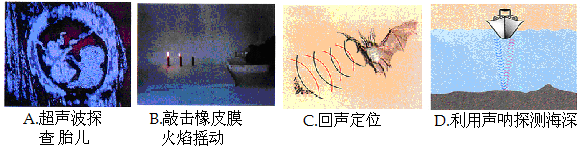
\includegraphics[scale=0.95]{figures/图片1.png} 


\question
利用超声波可测海洋的深度,已知声波在海水中的传播速度是$1500m/s$,若船上发出信号$6$秒钟后在海面收到反射回来的波,求海底的深度是多少?
\begin{solution}[8ex]
解:$h=s=vt/2=1500m/s \times 6s  \div 2=4500m$
\end{solution}


\question
一辆汽车朝山崖匀速行驶,在离山崖$700m$处鸣笛,汽车直线向前行驶$40m$后,司机刚好听到刚才鸣笛的回声。已知声音在空气中的传播速度是$340m/s$ ,求汽车行驶的速度。
\begin{solution}[12ex]
解:根据题意可知:\\
$t_\textrm{车}=t_\textrm{声} \\
t_\textrm{声}=s/v=(700m \times 2 -40m) \div 340m/s =4s\\ 
V_\textrm{车}=S_\textrm{车}/ t_\textrm{车}=40m/4s=10m/s$
\end{solution}

\question
反坦克炮瞄准一敌人的坦克,开炮后$0.6s$看到炮弹在敌坦克上爆炸,再经$2.1s$才听到爆声,若当时的声速为$340m/s$,则此反坦克炮距离敌坦克有多远?炮弹飞行的速度为多大?
\begin{solution}[12ex]
解:根据题意可知:\\
$0.6s$是炮弹用的时间,$2.1s$是声用的时间。\\
$S=v_\textrm{声}t_\textrm{声}=340m/s \times 2.1s =714m\\     
V_\textrm{炮}=S/t_\textrm{炮}=714m\div 0.6s=1190m/s$
\end{solution}




\end{questions}
\end{Aquestions}


\begin{Bquestions}
\newpage
\section{一般题}
\end{Bquestions}




\begin{Cquestions}
\newpage
\section{难题}
\end{Cquestions}



\begin{Dquestions}
\newpage
\section{中考题}
\end{Dquestions}




%
\ThisCenterWallPaper{1}{教案模板-3.pdf}

\end{document}



